\chapter{Grundlagen}
In diesem Kapitel sollen die für das weitere Verständnis notwendigen theoretischen Grundlagen erläutert werden. Dazu gehört zunächst der Aufbau des Netzwerks in einem Fahrzeug. Des Weiteren werden relevante Grundlagen der Cyber Security erklärt.

\section{Automotive Networking}
Im Inneren von Autos befinden sich heutzutage eine Vielzahl elektronischer Systeme, von denen jedes mit benachbarten Komponenten kommunizieren kann. Die einzelnen elektronischen Systeme werden als \acp{ECU} bezeichnet. Moderne Autos enthalten in der Regel über 50 verschiedene \acsp{ECU} \cite[vgl.][6]{Miller.2013}. Da diese Kontrolleinheiten zum Teil lebensentscheidende Aufgaben übernehmen, muss die Kommunikation zwischen den Einheiten möglichst in Echtzeit erfolgen. \\

\begin{figure}[H]
\centering
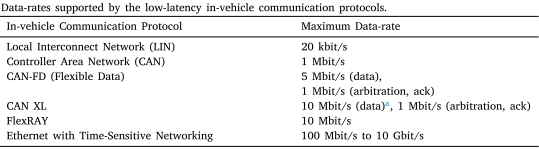
\includegraphics[width=\textwidth]{communication-protocols}
\label{fig:communication-protocols}
\caption{Verschiedene Kommunikationsprotokolle in Automobil-Netzwerken}
\quelle{\cite[2]{MohammadAshjaei.2021}}
\end{figure}

Für die Venetzung der \acsp{ECU} kommen verschiedene Technologien zum Einsatz (siehe Abbildung \ref{fig:communication-protocols}). Diese werden im Folgenden genauer erläutert. Die relevanteste davon ist im Automotive-Bereich der sogenannte \acs{CAN}-Standard.

\subsection{Controller Area Network}
Die elektronischen Kontrolleinheiten eines Autos sind typischerweise über einen oder mehrere Busse, die auf dem \ac{CAN}-Standard basieren, miteinander verbunden. Hierbei kommunizieren die \acsp{ECU} über \acs{CAN}-Pakete. Diese werden an alle Komponenten gesendet, welche dann jeweils basierend auf dem Inhalt entscheiden, ob das Paket für sie bestimmt ist oder nicht. Eine Identifikation der Quelle oder Authentisierung gibt es in diesem Standard nicht. \cite[vgl.][7]{Miller.2013} \\
In Abbildung \ref{fig:canbus-ford2010} ist das \acs{CAN}-Netzwerk eines 2010 Ford Escape dargestellt. Das abgebildete Netzwerk verfügt über zwei Busse, einen medium speed (MS) und einen high speed (HS) \acs{CAN}-Bus. Beide Busse enden hier im \ac{DLC} (siehe Kapitel \ref{OBD-II}).
In Automotive Netzwerken lassen sich zwei Arten von \acs{CAN}-Paketen finden: normale \acs{CAN}-Pakete und diagnostische \acs{CAN}-Pakete. 

\begin{figure}[h]
\centering
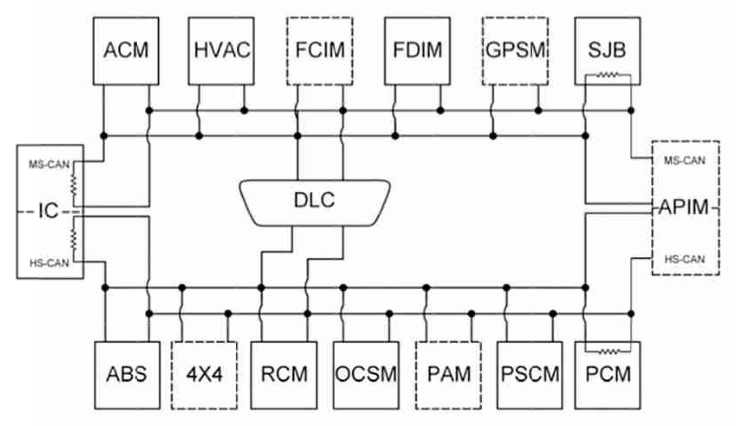
\includegraphics[width=\textwidth]{Miller_canbus-ford2010}
\label{fig:canbus-ford2010}
\caption{Beispiel des \acs{CAN}-Netzwerks eines 2010 Ford Escape}
\quelle{\cite[19]{Miller.2013}}
\end{figure}

\subsubsection{Normale \acs{CAN}-Pakete}
Normale Pakete werden von \acsp{ECU} gesendet und können entweder Informationen oder Befehle enthalten. Typischerweise werden sie alle Millisekunden gesendet. Auf Anwendungsebene enthalten die \acs{CAN}-Pakete einen Identifier, die zu übertragenden Daten und manchmal noch eine Prüfsumme, um sicherzustellen, dass das Paket korrekt übertragen wurde. Der Identifier gibt sowohl an, für welche \acsp{ECU} das Paket bestimmt ist, als auch, welche Priorität das Paket hat. \cite[vgl.][9]{Miller.2013}

\subsubsection{Diagnostische \acs{CAN}-Pakete}
Diagnostische Pakete tauchen während des normalen Betriebs des Autos im Normalfall nicht auf. Sie werden von Diagnose-Werkzeugen gesendet, die beispielsweise von Mechanikern genutzt werden um mit den \acsp{ECU} im Auto zu kommunizieren. So können Mängel und Fehlfunktionen entdeckt oder andere Informationen gewonnen werden. Das Format von diagnostischen \acs{CAN}-Paketen ähnelt dem von normalen Paketen, erfolgt jedoch meist nach strengeren Konventionen. Standards hierfür sind zum Beispiel ISO-TP, ISO 14229 und ISO 14230. \cite[vgl.][10]{Miller.2013}

\subsection{Local Interconnect Network}
Ein weiteres relevantes Protokoll im Automotive Bereich ist das \ac{LIN} Protokoll. Es wurde 1998 in Zusammenarbeit von Audi, BMW, DaimlerChrysler, Volvo, Volkswagen, VCT und Motorola entwickelt mit dem Ziel, ein möglichst kosteneffizientes Kommunikationsprotokoll zu schaffen \cite[57]{Fijalkowski.2011}.
Das \acs{LIN}-Protokoll basiert auf dem Serial Connections Interface Datenformat und ist in einer Single Master/Multiple Slaves Architektur aufgebaut. Das bedeutet, dass eine elektronische Kontrolleinheit als Masterknoten fungiert und andere elektronische Slave-Einheiten miteinander verbindet.
%Genauere Funktionsweise / Paketaufbau ergänzen

\subsubsection{Aufbau}
Nachrichtenpakete bestehen im \acs{LIN}-Standard aus einem Header und einem Data Frame. Der Header enthält einen Synchronisation Break, ein Synchronisation Byte und einen Message Identifier. Die ersten beiden Bestandteile sind für die Nachrichtensynchronisierung notwendig. Der Identifier wird benötigt, damit Knoten erkennen können, ob eine Nachricht für sie bestimmt ist. Der Data Frame ist nach dem 8N1-Schema aufgebaut. Das bedeutet, dass jedes Paket ein Startbit, acht Datenbits, kein Paritätsbit und ein Stopbit besitzt. \cite[58]{Fijalkowski.2011} \\
Im \acs{LIN}-Standard sind drei Arten von Kommunikation erlaubt.
\begin{enumerate}
\item Master to Slave, beziehungsweise Master to Multiple Slaves
\item Slave to Master
\item Slave to Slave
\end{enumerate}
Die Slaves können somit auch untereinander ohne Beiteiligung des Masters kommunizieren. \cite[59]{Fijalkowski.2011}

\subsubsection{Anwendung}
\ac{LIN} zeichnet sich wie oben erwähnt vor allem durch seine Kosteneffizienz aus. Allerdings bietet das Protokoll deutlich weniger Bandbreite als \acs{CAN}. Somit wird es vor allem an Stellen im Fahrzeug eingesetzt, wo nicht viel Bandbreite notwendig ist. Beispielsweise wird \acs{LIN} häufig für die Steuerung von Türen, Dach, Sitzen und dem Lenkrad verwendet. \cite[59]{Fijalkowski.2011} \\
Für den Aufbau eines Netzwerks mit den zwei Protokollen gibt es zwei gängige Ansätze:
\begin{enumerate}
\item Mehrere \acsp{ECU} werden über \acs{LIN} mit einer zentralen \acs{ECU} verbunden. Die Verbindung dieser zentralen \acsp{ECU} erfolgt mit dem \acs{CAN}-Standard.
\item Alle \acsp{ECU} werden über \acs{LIN} mit einer zentralen \acs{ECU} verbunden.
\end{enumerate}
Der zweite Ansatz ist skalierbarer, da ohne großen Aufwand neue Knoten hinzugefügt werden können. Der erste Ansatz ermöglicht jedoch eine deutlich höhere Bandbreite bei der Kommunikation zwischen den Einheiten. \cite[58]{Fijalkowski.2011}


\subsection{Schnittstellen}
\subsubsection{OBD-II Port} \label{OBD-II}

\section{Cyber Security}
\subsection{Security Lifecycle}
\cite{Wurm.2022}
\subsection{ISMS}


\chapter{Angriffsflächen}
\subsection{Bootvorgang}
\cite{Wurm.2022}


\chapter{Schutzmaßnahmen}
\subsection{SecureBoot}
\cite{Wurm.2022}[84]